\section{Additional tools and Complements}

\begin{frame}[fragile]
  \frametitle{Unifying view of variables and individuals}

  \begin{block}{Principal components}
   The full matrix of principal component connects  individual coordinates to latent factors:
    \begin{equation*}
      \mathrm{PC} = \bX^c \bU = \begin{pmatrix}
      \mathbf{f}_{1} & \mathbf{f}_{2} & \dots & \mathbf{f}_{d}
      \end{pmatrix}
      = \begin{pmatrix} 
      \bc_{1}^\top \\ \bc_{2}^\top \\\dots \\ \bc_{d}^\top 
      \end{pmatrix}
    \end{equation*}
  \end{block}

  \vfill
  
  \begin{itemize}
    \item new variables (latent factor) are seen column-wise
    \item new coordinates are seen row-wise
  \end{itemize}

  $\rightsquigarrow$ Everything can be interpreted on a single plot, called the biplot

\end{frame}

\begin{frame}[fragile]
  \frametitle{Biplot (1)}
\begin{knitrout}
\definecolor{shadecolor}{rgb}{0.969, 0.969, 0.969}\color{fgcolor}\begin{kframe}
\begin{alltt}
\hlstd{FactoMineR}\hlopt{::}\hlkwd{PCA}\hlstd{(}\hlkwd{select}\hlstd{(crabs,} \hlopt{-}\hlstd{species,} \hlopt{-}\hlstd{sex),} \hlkwc{scale.unit} \hlstd{=} \hlnum{FALSE}\hlstd{,} \hlkwc{graph} \hlstd{=} \hlnum{FALSE}\hlstd{)} \hlopt
  \hlstd{factoextra}\hlopt{::}\hlkwd{fviz_pca_biplot}\hlstd{(}
    \hlkwc{axes} \hlstd{=} \hlkwd{c}\hlstd{(}\hlnum{1}\hlstd{,}\hlnum{2}\hlstd{),} \hlkwc{col.ind} \hlstd{=} \hlkwd{paste}\hlstd{(crabs}\hlopt{$}\hlstd{species, crabs}\hlopt{$}\hlstd{sex),} \hlkwc{palette} \hlstd{= pal}
  \hlstd{)}
\end{alltt}


{\ttfamily\noindent\bfseries\color{errorcolor}{\#\# Error in FactoMineR::PCA(select(crabs, -species, -sex), scale.unit = FALSE, : could not find function "{}\%>\%"{}}}\end{kframe}
\end{knitrout}
\end{frame}

\begin{frame}[fragile]
  \frametitle{Biplot (2)}
\begin{knitrout}
\definecolor{shadecolor}{rgb}{0.969, 0.969, 0.969}\color{fgcolor}\begin{kframe}
\begin{alltt}
\hlstd{FactoMineR}\hlopt{::}\hlkwd{PCA}\hlstd{(}\hlkwd{select}\hlstd{(crabs,} \hlopt{-}\hlstd{species,} \hlopt{-}\hlstd{sex),} \hlkwc{scale.unit} \hlstd{=} \hlnum{FALSE}\hlstd{,} \hlkwc{graph} \hlstd{=} \hlnum{FALSE}\hlstd{)} \hlopt
  \hlstd{factoextra}\hlopt{::}\hlkwd{fviz_pca_biplot}\hlstd{(}
    \hlkwc{axes} \hlstd{=} \hlkwd{c}\hlstd{(}\hlnum{2}\hlstd{,}\hlnum{3}\hlstd{),} \hlkwc{col.ind} \hlstd{=} \hlkwd{paste}\hlstd{(crabs}\hlopt{$}\hlstd{species, crabs}\hlopt{$}\hlstd{sex),} \hlkwc{palette} \hlstd{= pal}
  \hlstd{)}
\end{alltt}


{\ttfamily\noindent\bfseries\color{errorcolor}{\#\# Error in FactoMineR::PCA(select(crabs, -species, -sex), scale.unit = FALSE, : could not find function "{}\%>\%"{}}}\end{kframe}
\end{knitrout}
\end{frame}

\begin{frame}
  \frametitle{Reconstruction formula}

    Recall that $\mathbf{F} = (\mathbf{f}_1, \dots, \mathbf{f}_d) $ is the matrix of Principal components. Then,  
    \begin{itemize}
      \item  $\mathbf{f}_k = \bX^c \bu_k$ for projection on axis $k$
      \item $\mathbf{F} = \bX^c \bU$ for all axis.
    \end{itemize}
    Using orthogonality of $\bU$, we get back the original data as follows, without loss ($\bU^T$ performs the inverse rotation of $\bU$):
    \begin{equation*}
      \bX^c = \mathbf{F}\bU^\top 
    \end{equation*}

    \vfill
    \pause 
    
    We obtain an approximation $\tilde\bX^c$ (compression) of the data $\bX^c$ by considering a subset $\mathcal{S}$ of PC, typically $\mathcal{S} = {1, \dots,K}$ with $K \ll d$.
    \begin{equation*}
      \tilde\bX^c = \mathbf{F}_{\mathcal{S}}\bU_{\mathcal{S}}^\top = \bX^c \bU_{\mathcal{S}} \bU_{\mathcal{S}}^\top
    \end{equation*}
    $\rightsquigarrow$ This is a rank $K$ approximation of $\bX$ of the data the information capture by the first $K$ axes.

\end{frame}

\begin{frame}[fragile,allowframebreaks]
  \frametitle{Remove size effect}
  \framesubtitle{Carried by the 1st principal component}

\paragraph{First component}
\begin{equation*}
  \mathbf{f}_1 = \mathbf{X}^c \mathbf{u}_1.
\end{equation*}

We extract the best rank-1 approximation of $\mathbf{X}$ to remove the \textit{size effect}, carried by the first axis, and return to the original space,
\begin{equation*}
  \tilde{\mathbf{X}}^{(1)} = \mathbf{f}_1 \mathbf{u}_1^\top.
\end{equation*}


\begin{knitrout}
\definecolor{shadecolor}{rgb}{0.969, 0.969, 0.969}\color{fgcolor}\begin{kframe}
\begin{alltt}
\hlstd{attributes} \hlkwb{<-} \hlkwd{select}\hlstd{(crabs,} \hlopt{-}\hlstd{sex,} \hlopt{-}\hlstd{species)} \hlopt \hlkwd{as.matrix}\hlstd{()}
\end{alltt}


{\ttfamily\noindent\bfseries\color{errorcolor}{\#\# Error in select(crabs, -sex, -species) \%>\% as.matrix(): could not find function "{}\%>\%"{}}}\begin{alltt}
\hlstd{u1} \hlkwb{<-} \hlkwd{eigen}\hlstd{(}\hlkwd{cov}\hlstd{(attributes))}\hlopt{$}\hlstd{vectors[,} \hlnum{1}\hlstd{,} \hlkwc{drop} \hlstd{=} \hlnum{FALSE}\hlstd{]}
\end{alltt}


{\ttfamily\noindent\bfseries\color{errorcolor}{\#\# Error in cov(attributes): supply both 'x' and 'y' or a matrix-like 'x'}}\begin{alltt}
\hlstd{attributes_rank1} \hlkwb{<-} \hlstd{attributes} \hlopt \hlstd{u1} \hlopt \hlkwd{t}\hlstd{(u1)}
\end{alltt}


{\ttfamily\noindent\bfseries\color{errorcolor}{\#\# Error in eval(expr, envir, enclos): object 'u1' not found}}\begin{alltt}
\hlstd{crabs_corrected} \hlkwb{<-} \hlstd{crabs}
\end{alltt}


{\ttfamily\noindent\bfseries\color{errorcolor}{\#\# Error in eval(expr, envir, enclos): object 'crabs' not found}}\begin{alltt}
\hlstd{crabs_corrected[,} \hlnum{3}\hlopt{:}\hlnum{7}\hlstd{]} \hlkwb{<-} \hlstd{attributes} \hlopt{-} \hlstd{attributes_rank1}
\end{alltt}


{\ttfamily\noindent\bfseries\color{errorcolor}{\#\# Error in eval(expr, envir, enclos): object 'attributes\_rank1' not found}}\end{kframe}
\end{knitrout}

$\rightsquigarrow$ Axis 1 explains a latent effect, here the size in the case at hand, common to all attributes.

\begin{knitrout}
\definecolor{shadecolor}{rgb}{0.969, 0.969, 0.969}\color{fgcolor}\begin{kframe}
\begin{alltt}
\hlkwd{ggpairs}\hlstd{(crabs_corrected,} \hlkwc{columns} \hlstd{=} \hlnum{3}\hlopt{:}\hlnum{7}\hlstd{,} \hlkwd{aes}\hlstd{(}\hlkwc{colour} \hlstd{= species,} \hlkwc{shape} \hlstd{= sex))}
\end{alltt}


{\ttfamily\noindent\bfseries\color{errorcolor}{\#\# Error in ggpairs(crabs\_corrected, columns = 3:7, aes(colour = species, : could not find function "{}ggpairs"{}}}\end{kframe}
\end{knitrout}

\end{frame}

\begin{frame}[fragile]
  \frametitle{PCA on corrected data (1)}
\begin{knitrout}
\definecolor{shadecolor}{rgb}{0.969, 0.969, 0.969}\color{fgcolor}\begin{kframe}
\begin{alltt}
\hlstd{crabs_pca_corrected} \hlkwb{<-} \hlkwd{select}\hlstd{(crabs_corrected,} \hlopt{-}\hlstd{species,} \hlopt{-}\hlstd{sex)} \hlopt \hlstd{FactoMineR}\hlopt{::}\hlkwd{PCA}\hlstd{(}\hlkwc{graph} \hlstd{=} \hlnum{FALSE}\hlstd{)}
\end{alltt}


{\ttfamily\noindent\bfseries\color{errorcolor}{\#\# Error in select(crabs\_corrected, -species, -sex) \%>\% FactoMineR::PCA(graph = FALSE): could not find function "{}\%>\%"{}}}\begin{alltt}
\hlkwd{fviz_eig}\hlstd{(crabs_pca_corrected)}
\end{alltt}


{\ttfamily\noindent\bfseries\color{errorcolor}{\#\# Error in fviz\_eig(crabs\_pca\_corrected): could not find function "{}fviz\_eig"{}}}\end{kframe}
\end{knitrout}
\end{frame}

\begin{frame}[fragile]
  \frametitle{PCA on corrected data (2)}
\begin{knitrout}
\definecolor{shadecolor}{rgb}{0.969, 0.969, 0.969}\color{fgcolor}\begin{kframe}
\begin{alltt}
\hlkwd{fviz_pca_ind}\hlstd{(crabs_pca_corrected,} \hlkwc{col.ind} \hlstd{=} \hlkwd{paste}\hlstd{(crabs_corrected}\hlopt{$}\hlstd{species, crabs_corrected}\hlopt{$}\hlstd{sex),} \hlkwc{palette} \hlstd{= pal)}
\end{alltt}


{\ttfamily\noindent\bfseries\color{errorcolor}{\#\# Error in fviz\_pca\_ind(crabs\_pca\_corrected, col.ind = paste(crabs\_corrected\$species, : could not find function "{}fviz\_pca\_ind"{}}}\end{kframe}
\end{knitrout}
\end{frame}

\begin{frame}[fragile]
  \frametitle{PCA on corrected data (3)}
\begin{knitrout}
\definecolor{shadecolor}{rgb}{0.969, 0.969, 0.969}\color{fgcolor}\begin{kframe}
\begin{alltt}
\hlkwd{fviz_pca_var}\hlstd{(crabs_pca_corrected,} \hlkwc{col.var} \hlstd{=} \hlstr{'cos2'}\hlstd{)}
\end{alltt}


{\ttfamily\noindent\bfseries\color{errorcolor}{\#\# Error in fviz\_pca\_var(crabs\_pca\_corrected, col.var = "{}cos2"{}): could not find function "{}fviz\_pca\_var"{}}}\end{kframe}
\end{knitrout}
\end{frame}

\begin{frame}[fragile]
  \frametitle{PCA on corrected data (3)}
\begin{knitrout}
\definecolor{shadecolor}{rgb}{0.969, 0.969, 0.969}\color{fgcolor}\begin{kframe}
\begin{alltt}
\hlkwd{fviz_pca_biplot}\hlstd{(crabs_pca_corrected,} \hlkwc{col.ind} \hlstd{=} \hlkwd{paste}\hlstd{(crabs_corrected}\hlopt{$}\hlstd{species, crabs_corrected}\hlopt{$}\hlstd{sex),} \hlkwc{palette} \hlstd{= pal)}
\end{alltt}


{\ttfamily\noindent\bfseries\color{errorcolor}{\#\# Error in fviz\_pca\_biplot(crabs\_pca\_corrected, col.ind = paste(crabs\_corrected\$species, : could not find function "{}fviz\_pca\_biplot"{}}}\end{kframe}
\end{knitrout}
\end{frame}

\begin{frame}
  \frametitle{Choosing the number of components}

  \begin{columns}
  \begin{column}{0.68\textwidth}
    \begin{block}{Various solutions, open question}
    Scree plot, test on eigenvalues, confidence interval, cross-validation, generalized cross-validation, etc.
    \end{block}
  \end{column}~~
  \begin{column}{0.3\textwidth}
    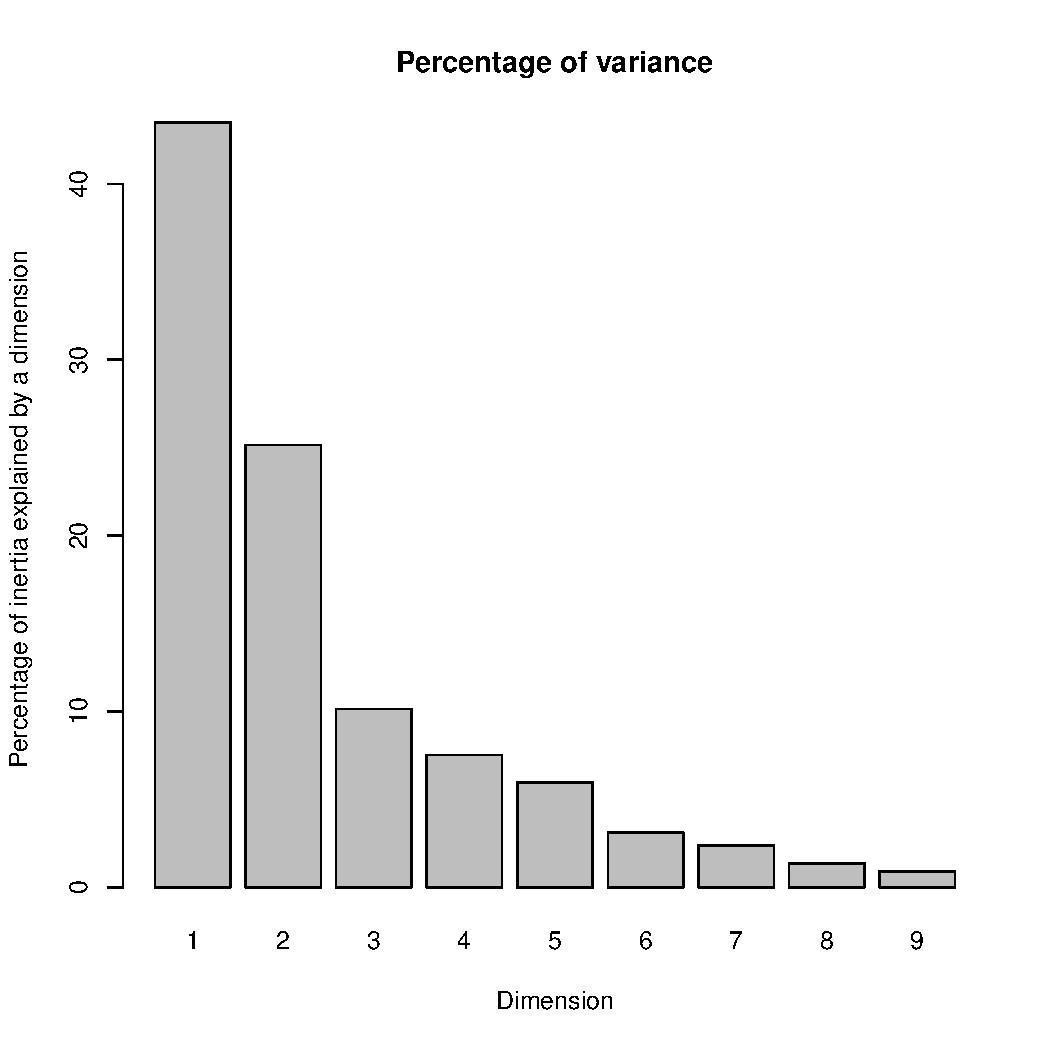
\includegraphics[width=\textwidth]{wine_pca_eig}
  \end{column}
  \end{columns}
  
  \begin{columns}
  \begin{column}{.5\textwidth}
  \begin{block}{Objectives}
    \begin{itemize}
      \item Interpretation
      \item Separate structure and noise
      \item Data compression    
    \end{itemize}
  \end{block}
\end{column}
\begin{column}{0.5\textwidth}
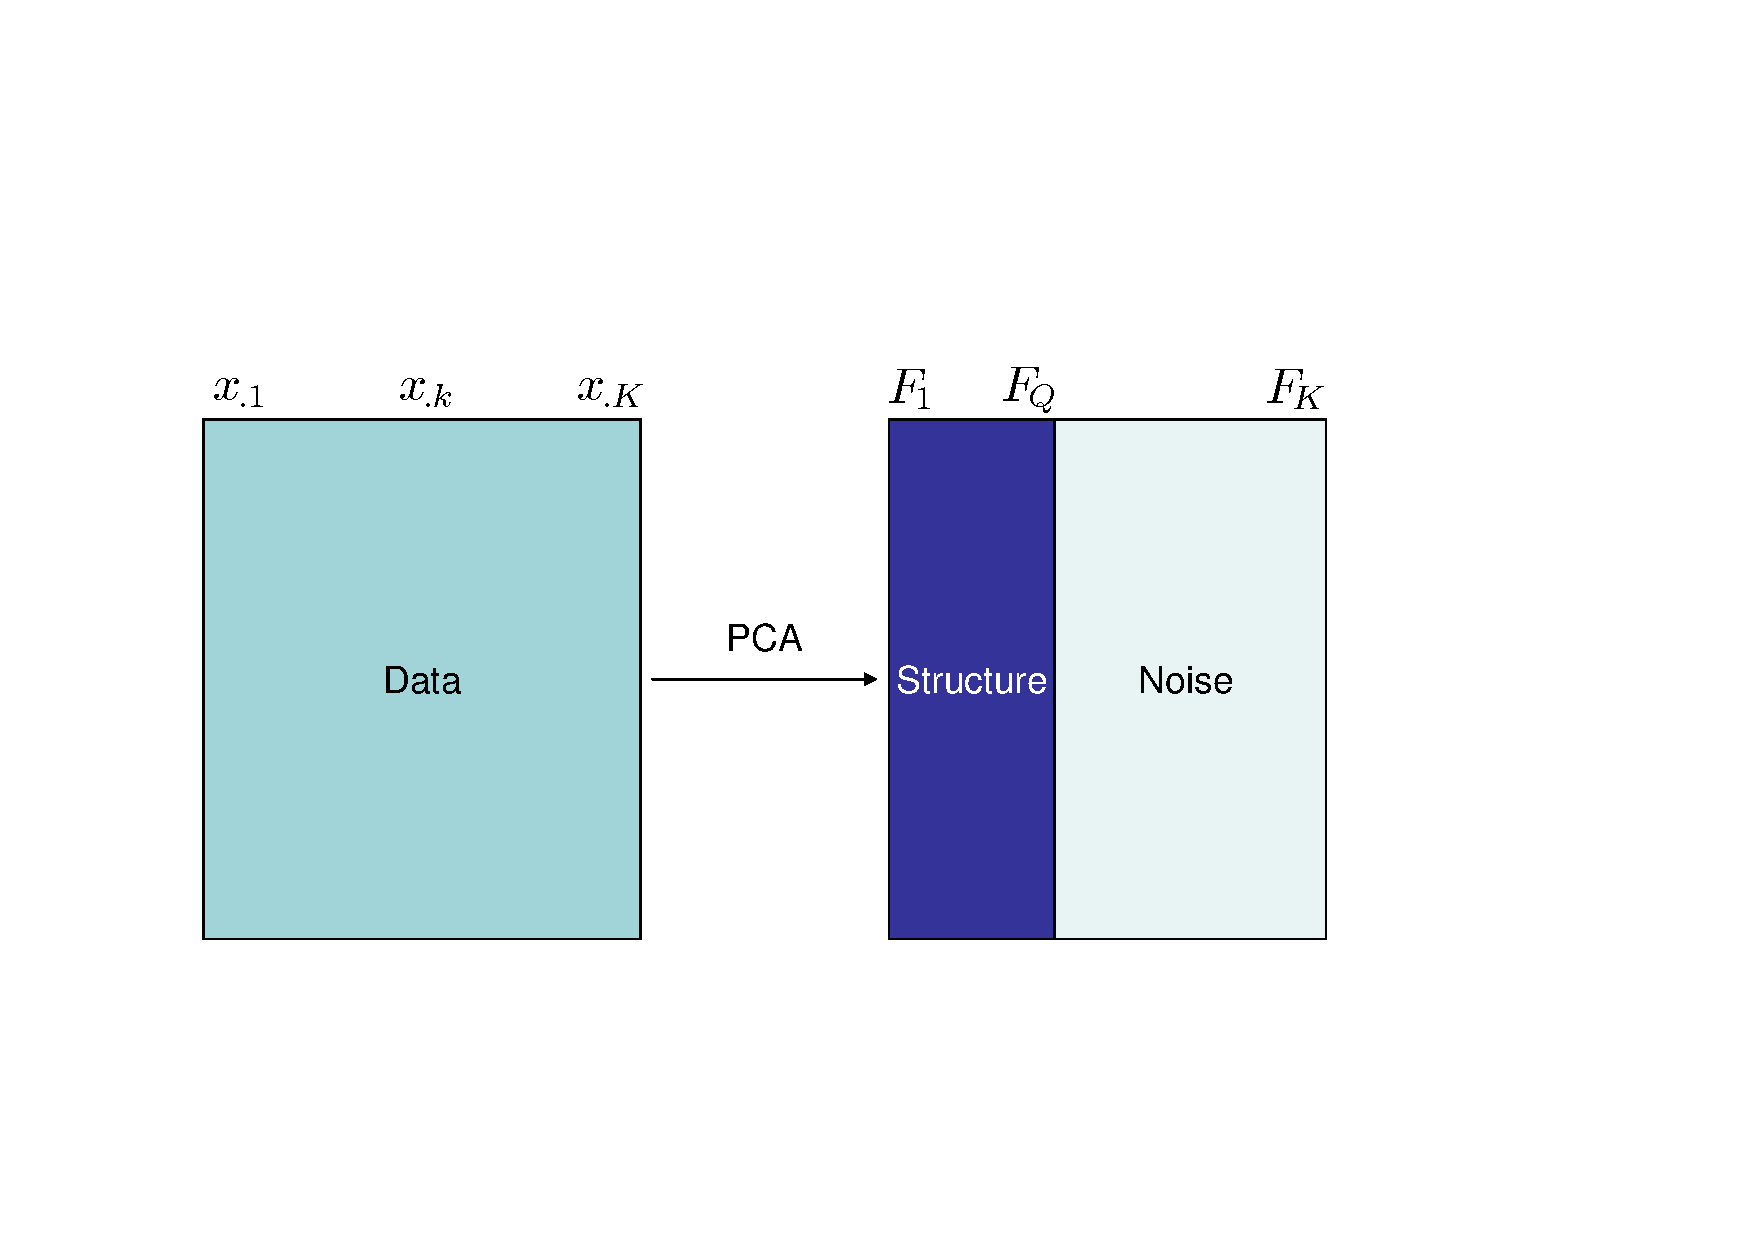
\includegraphics[width=\textwidth]{dim_reduc.pdf}
  \end{column}
  \end{columns}
\end{frame}

\begin{frame}[fragile]
  \frametitle{Example: Generalized Cross Validation}

\begin{knitrout}
\definecolor{shadecolor}{rgb}{0.969, 0.969, 0.969}\color{fgcolor}\begin{kframe}
\begin{alltt}
\hlstd{GCV} \hlkwb{<-} \hlkwd{select}\hlstd{(crabs_corrected,} \hlopt{-}\hlstd{species,} \hlopt{-}\hlstd{sex)} \hlopt
  \hlstd{FactoMineR}\hlopt{::}\hlkwd{estim_ncp}\hlstd{(}\hlkwc{ncp.min} \hlstd{=} \hlnum{1}\hlstd{,} \hlkwc{ncp.max} \hlstd{=} \hlnum{4}\hlstd{)}
\end{alltt}


{\ttfamily\noindent\bfseries\color{errorcolor}{\#\# Error in select(crabs\_corrected, -species, -sex) \%>\% FactoMineR::estim\_ncp(ncp.min = 1, : could not find function "{}\%>\%"{}}}\begin{alltt}
\hlkwd{qplot}\hlstd{(}\hlnum{1}\hlopt{:}\hlkwd{length}\hlstd{(GCV}\hlopt{$}\hlstd{criterion), GCV}\hlopt{$}\hlstd{criterion,} \hlkwc{geom} \hlstd{=} \hlstr{"line"}\hlstd{)} \hlopt{+} \hlkwd{labs}\hlstd{(}\hlstr{"number of axis"}\hlstd{,} \hlstr{"GCV"}\hlstd{)}
\end{alltt}


{\ttfamily\noindent\bfseries\color{errorcolor}{\#\# Error in qplot(1:length(GCV\$criterion), GCV\$criterion, geom = "{}line"{}): could not find function "{}qplot"{}}}\end{kframe}
\end{knitrout}
\end{frame}

\begin{frame}
\frametitle{Supplementary information}
\vfill
\begin{itemize}
\item continuous variables: projection (correlation with dimensions)
\item observations: projection
\item categorical variables: projection of the categories at the barycentre of the observations which take the categories
\begin{figure}[H]
  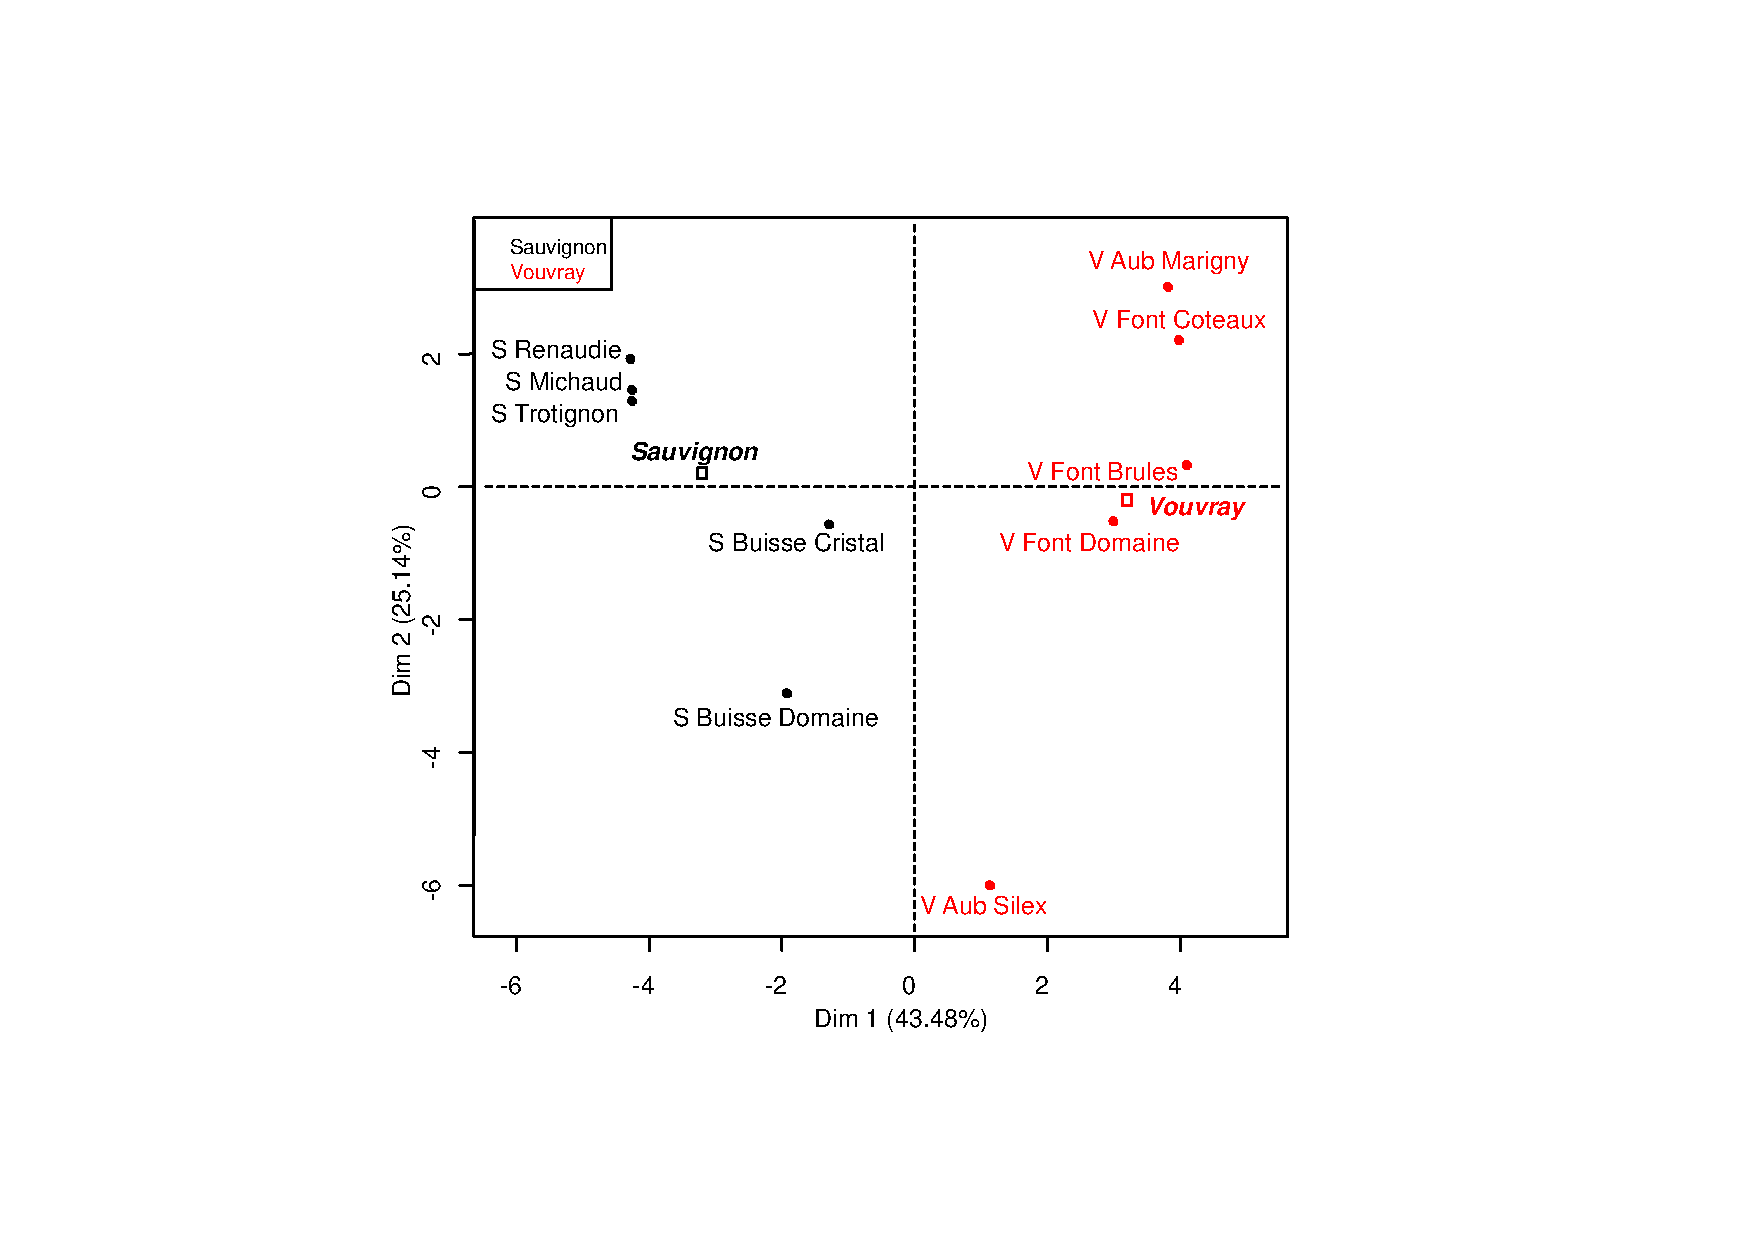
\includegraphics[width=0.4\textwidth]{wine_PCA_ind_mod_coul.pdf}~~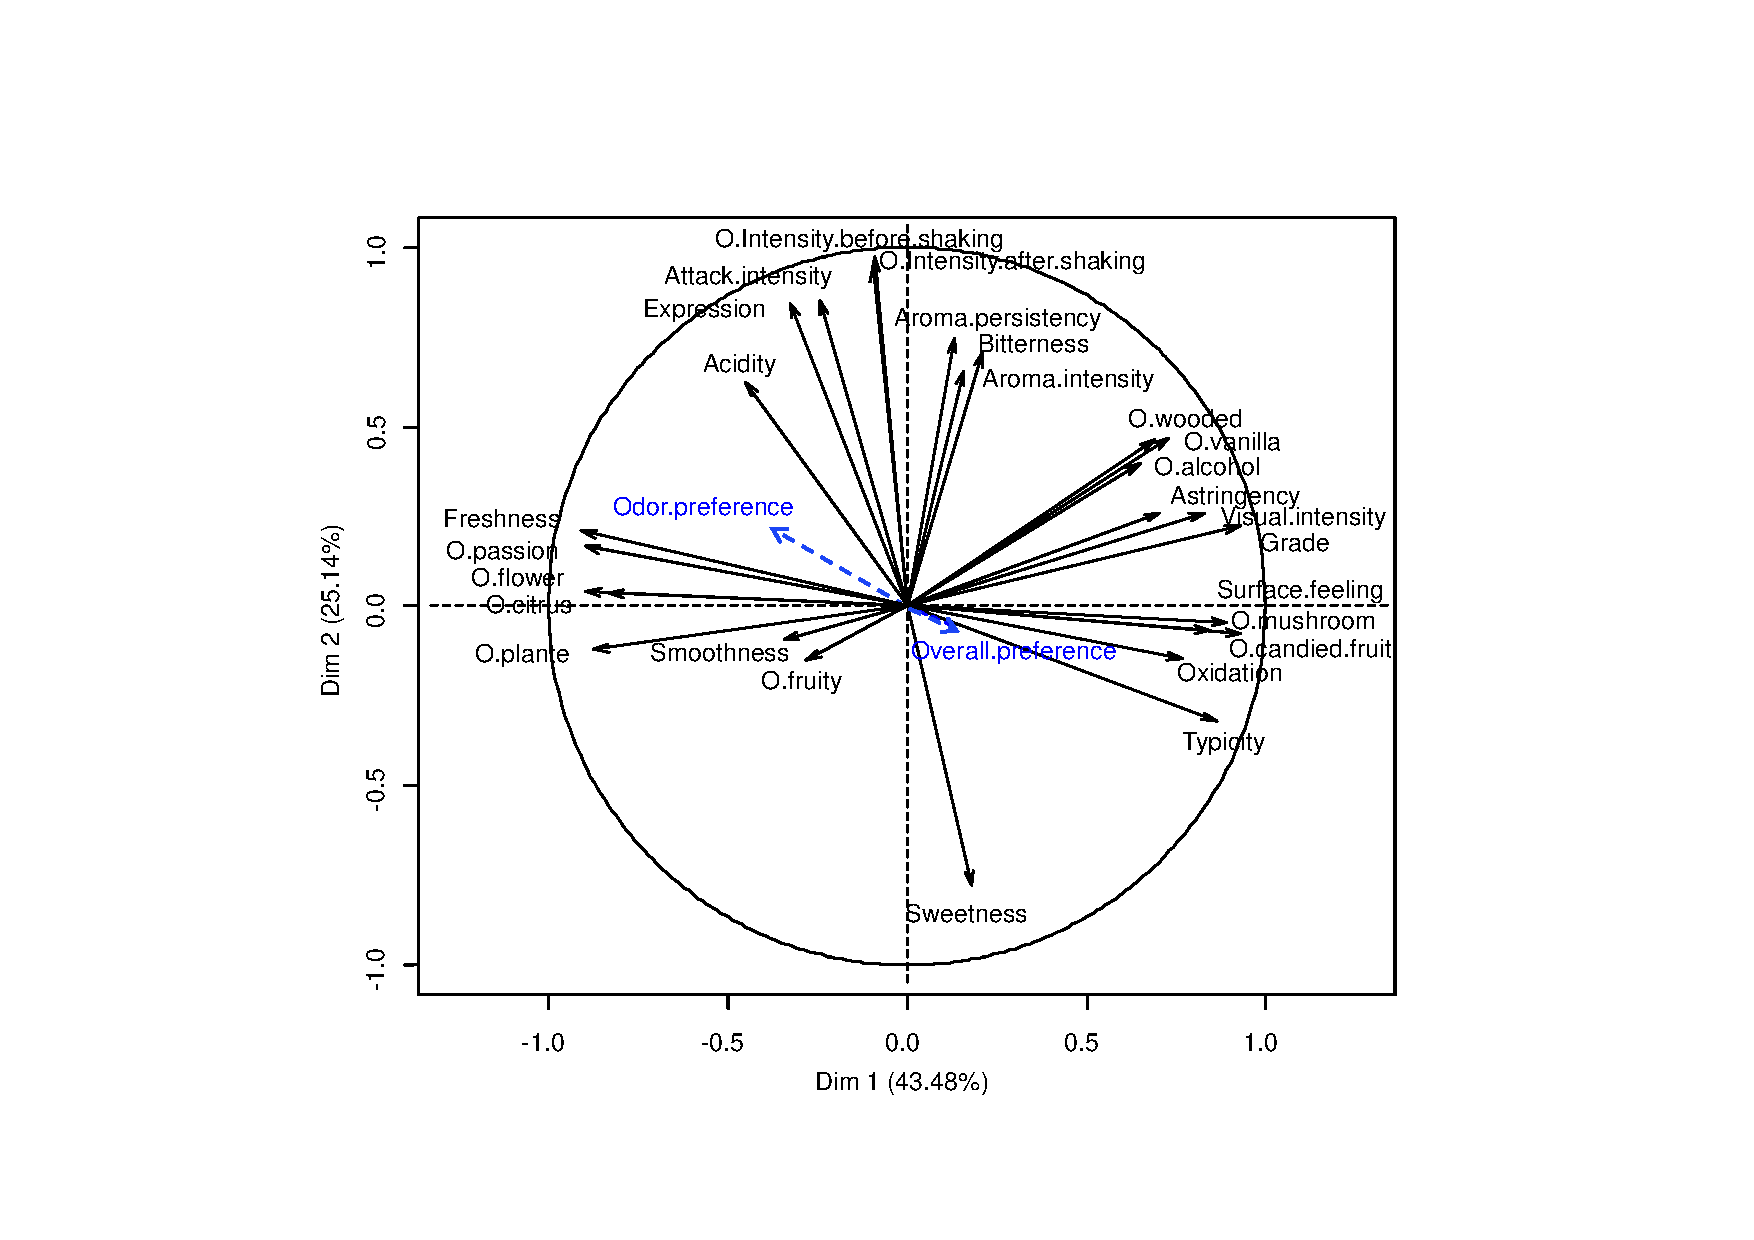
\includegraphics[width=0.55\textwidth]{wine_PCA_var_supp.pdf}
\end{figure}
\end{itemize}
\end{frame}


\begin{frame}[fragile]
\frametitle{Description of  dimensions}
  
  \begin{block}{Using continuous variables}
    \begin{itemize}
      \item correlation between variable and the principal components
      \item sort correlation coefficients and give significant ones (rought tests)
    \end{itemize}
  \end{block}
  
  \begin{block}{Using categorical variables}
    One-way anova with the coordinates of the observations ($F_{.q}$) explained by the categorical variable
    \begin{itemize}
      \item F-test by variable
      \item for each category, a Student's $T$-test to compare the average of the category with the general mean
    \end{itemize}
  \end{block}

\end{frame}

\begin{frame}[fragile, allowframebreaks]
\frametitle{Description of  dimensions: example}

\begin{knitrout}
\definecolor{shadecolor}{rgb}{0.969, 0.969, 0.969}\color{fgcolor}\begin{kframe}
\begin{alltt}
\hlstd{crabs_pca_corrected} \hlkwb{<-} \hlstd{crabs_corrected} \hlopt \hlstd{FactoMineR}\hlopt{::}\hlkwd{PCA}\hlstd{(}\hlkwc{graph} \hlstd{=} \hlnum{FALSE}\hlstd{,} \hlkwc{quali.sup} \hlstd{=} \hlkwd{c}\hlstd{(}\hlnum{1}\hlstd{,}\hlnum{2}\hlstd{))}
\end{alltt}


{\ttfamily\noindent\bfseries\color{errorcolor}{\#\# Error in crabs\_corrected \%>\% FactoMineR::PCA(graph = FALSE, quali.sup = c(1, : could not find function "{}\%>\%"{}}}\begin{alltt}
\hlstd{FactoMineR}\hlopt{::}\hlkwd{dimdesc}\hlstd{(crabs_pca_corrected)}
\end{alltt}


{\ttfamily\noindent\bfseries\color{errorcolor}{\#\# Error in FactoMineR::dimdesc(crabs\_pca\_corrected): object 'crabs\_pca\_corrected' not found}}\end{kframe}
\end{knitrout}

\end{frame}
